\documentclass[twoside]{book}

% Packages required by doxygen
\usepackage{fixltx2e}
\usepackage{calc}
\usepackage{doxygen}
\usepackage[export]{adjustbox} % also loads graphicx
\usepackage{graphicx}
\usepackage[utf8]{inputenc}
\usepackage{makeidx}
\usepackage{multicol}
\usepackage{multirow}
\PassOptionsToPackage{warn}{textcomp}
\usepackage{textcomp}
\usepackage[nointegrals]{wasysym}
\usepackage[table]{xcolor}

% Font selection
\usepackage[T1]{fontenc}
\usepackage[scaled=.90]{helvet}
\usepackage{courier}
\usepackage{amssymb}
\usepackage{sectsty}
\renewcommand{\familydefault}{\sfdefault}
\allsectionsfont{%
  \fontseries{bc}\selectfont%
  \color{darkgray}%
}
\renewcommand{\DoxyLabelFont}{%
  \fontseries{bc}\selectfont%
  \color{darkgray}%
}
\newcommand{\+}{\discretionary{\mbox{\scriptsize$\hookleftarrow$}}{}{}}

% Page & text layout
\usepackage{geometry}
\geometry{%
  a4paper,%
  top=2.5cm,%
  bottom=2.5cm,%
  left=2.5cm,%
  right=2.5cm%
}
\tolerance=750
\hfuzz=15pt
\hbadness=750
\setlength{\emergencystretch}{15pt}
\setlength{\parindent}{0cm}
\setlength{\parskip}{3ex plus 2ex minus 2ex}
\makeatletter
\renewcommand{\paragraph}{%
  \@startsection{paragraph}{4}{0ex}{-1.0ex}{1.0ex}{%
    \normalfont\normalsize\bfseries\SS@parafont%
  }%
}
\renewcommand{\subparagraph}{%
  \@startsection{subparagraph}{5}{0ex}{-1.0ex}{1.0ex}{%
    \normalfont\normalsize\bfseries\SS@subparafont%
  }%
}
\makeatother

% Headers & footers
\usepackage{fancyhdr}
\pagestyle{fancyplain}
\fancyhead[LE]{\fancyplain{}{\bfseries\thepage}}
\fancyhead[CE]{\fancyplain{}{}}
\fancyhead[RE]{\fancyplain{}{\bfseries\leftmark}}
\fancyhead[LO]{\fancyplain{}{\bfseries\rightmark}}
\fancyhead[CO]{\fancyplain{}{}}
\fancyhead[RO]{\fancyplain{}{\bfseries\thepage}}
\fancyfoot[LE]{\fancyplain{}{}}
\fancyfoot[CE]{\fancyplain{}{}}
\fancyfoot[RE]{\fancyplain{}{\bfseries\scriptsize Generated by Doxygen }}
\fancyfoot[LO]{\fancyplain{}{\bfseries\scriptsize Generated by Doxygen }}
\fancyfoot[CO]{\fancyplain{}{}}
\fancyfoot[RO]{\fancyplain{}{}}
\renewcommand{\footrulewidth}{0.4pt}
\renewcommand{\chaptermark}[1]{%
  \markboth{#1}{}%
}
\renewcommand{\sectionmark}[1]{%
  \markright{\thesection\ #1}%
}

% Indices & bibliography
\usepackage{natbib}
\usepackage[titles]{tocloft}
\setcounter{tocdepth}{3}
\setcounter{secnumdepth}{5}
\makeindex

% Hyperlinks (required, but should be loaded last)
\usepackage{ifpdf}
\ifpdf
  \usepackage[pdftex,pagebackref=true]{hyperref}
\else
  \usepackage[ps2pdf,pagebackref=true]{hyperref}
\fi
\hypersetup{%
  colorlinks=true,%
  linkcolor=blue,%
  citecolor=blue,%
  unicode%
}

% Custom commands
\newcommand{\clearemptydoublepage}{%
  \newpage{\pagestyle{empty}\cleardoublepage}%
}

\usepackage{caption}
\captionsetup{labelsep=space,justification=centering,font={bf},singlelinecheck=off,skip=4pt,position=top}

%===== C O N T E N T S =====

\begin{document}

% Titlepage & ToC
\hypersetup{pageanchor=false,
             bookmarksnumbered=true,
             pdfencoding=unicode
            }
\pagenumbering{alph}
\begin{titlepage}
\vspace*{7cm}
\begin{center}%
{\Large My Project }\\
\vspace*{1cm}
{\large Generated by Doxygen 1.8.13}\\
\end{center}
\end{titlepage}
\clearemptydoublepage
\pagenumbering{roman}
\tableofcontents
\clearemptydoublepage
\pagenumbering{arabic}
\hypersetup{pageanchor=true}

%--- Begin generated contents ---
\chapter{Data Structure Index}
\section{Data Structures}
Here are the data structures with brief descriptions\+:\begin{DoxyCompactList}
\item\contentsline{section}{\hyperlink{structEnemy}{Enemy} }{\pageref{structEnemy}}{}
\item\contentsline{section}{\hyperlink{structmaps}{maps} }{\pageref{structmaps}}{}
\item\contentsline{section}{\hyperlink{structObjet}{Objet} }{\pageref{structObjet}}{}
\item\contentsline{section}{\hyperlink{structperso}{perso} }{\pageref{structperso}}{}
\end{DoxyCompactList}

\chapter{File Index}
\section{File List}
Here is a list of all documented files with brief descriptions\+:\begin{DoxyCompactList}
\item\contentsline{section}{\hyperlink{coll_8c}{coll.\+c} \\*Collision parfaite $\ast$ }{\pageref{coll_8c}}{}
\item\contentsline{section}{{\bfseries coll.\+h} }{\pageref{coll_8h}}{}
\item\contentsline{section}{{\bfseries ennemi.\+h} }{\pageref{ennemi_8h}}{}
\item\contentsline{section}{{\bfseries file.\+h} }{\pageref{file_8h}}{}
\item\contentsline{section}{\hyperlink{jeu_8c}{jeu.\+c} \\*L\textquotesingle{}affichage du jeu $\ast$ }{\pageref{jeu_8c}}{}
\item\contentsline{section}{\hyperlink{main_8c}{main.\+c} \\*Le menu du jeu $\ast$ }{\pageref{main_8c}}{}
\item\contentsline{section}{{\bfseries main.\+h} }{\pageref{main_8h}}{}
\item\contentsline{section}{{\bfseries object.\+h} }{\pageref{object_8h}}{}
\item\contentsline{section}{{\bfseries per.\+h} }{\pageref{per_8h}}{}
\item\contentsline{section}{{\bfseries scrolling.\+h} }{\pageref{scrolling_8h}}{}
\end{DoxyCompactList}

\chapter{Data Structure Documentation}
\hypertarget{structEnemy}{}\section{Enemy Struct Reference}
\label{structEnemy}\index{Enemy@{Enemy}}
\subsection*{Data Fields}
\begin{DoxyCompactItemize}
\item 
\mbox{\Hypertarget{structEnemy_afc1cf868e4b6602d2166ee9cfbf1d06e}\label{structEnemy_afc1cf868e4b6602d2166ee9cfbf1d06e}} 
S\+D\+L\+\_\+\+Surface $\ast$ {\bfseries image} \mbox{[}3\mbox{]}
\item 
\mbox{\Hypertarget{structEnemy_a62ed00c1aa4ac7bb90cb132c6c56b21d}\label{structEnemy_a62ed00c1aa4ac7bb90cb132c6c56b21d}} 
S\+D\+L\+\_\+\+Surface $\ast$ {\bfseries Hit}
\item 
\mbox{\Hypertarget{structEnemy_ab8d7f9eceeef8f17331210f3f1fd2cf3}\label{structEnemy_ab8d7f9eceeef8f17331210f3f1fd2cf3}} 
S\+D\+L\+\_\+\+Surface $\ast$ {\bfseries image\+Actuel}
\item 
\mbox{\Hypertarget{structEnemy_ac364f2ddf130c8622889deca0b6ba4d0}\label{structEnemy_ac364f2ddf130c8622889deca0b6ba4d0}} 
S\+D\+L\+\_\+\+Rect {\bfseries position}
\item 
\mbox{\Hypertarget{structEnemy_a192ae3acb8bf84c4ecb81bf4864fc648}\label{structEnemy_a192ae3acb8bf84c4ecb81bf4864fc648}} 
int {\bfseries fram}
\item 
\mbox{\Hypertarget{structEnemy_a1de1605c4b41f74c3b0f4023258323ab}\label{structEnemy_a1de1605c4b41f74c3b0f4023258323ab}} 
int {\bfseries direction}
\end{DoxyCompactItemize}


The documentation for this struct was generated from the following file\+:\begin{DoxyCompactItemize}
\item 
file.\+h\end{DoxyCompactItemize}

\hypertarget{structmaps}{}\section{maps Struct Reference}
\label{structmaps}\index{maps@{maps}}
\subsection*{Data Fields}
\begin{DoxyCompactItemize}
\item 
\mbox{\Hypertarget{structmaps_aa31ebc131e955a0f360296f2511a3468}\label{structmaps_aa31ebc131e955a0f360296f2511a3468}} 
S\+D\+L\+\_\+\+Surface $\ast$ {\bfseries calque}
\item 
\mbox{\Hypertarget{structmaps_ab0ccde61b380fa3e3b50cfb958fa91de}\label{structmaps_ab0ccde61b380fa3e3b50cfb958fa91de}} 
int {\bfseries speed\+\_\+camera}
\item 
\mbox{\Hypertarget{structmaps_aab82595723041ff5880fe1605114c08a}\label{structmaps_aab82595723041ff5880fe1605114c08a}} 
S\+D\+L\+\_\+\+Rect {\bfseries camera}
\item 
\mbox{\Hypertarget{structmaps_adff29539db744060487f28ecf3850d00}\label{structmaps_adff29539db744060487f28ecf3850d00}} 
int {\bfseries buttoncameraup}
\item 
\mbox{\Hypertarget{structmaps_abdef6a37c6ff8d4a841f11efec2f2647}\label{structmaps_abdef6a37c6ff8d4a841f11efec2f2647}} 
S\+D\+L\+\_\+\+Surface $\ast$ {\bfseries affichage\+\_\+map}
\item 
\mbox{\Hypertarget{structmaps_aea036e289f40fb2cc9e0bb056f69c5c0}\label{structmaps_aea036e289f40fb2cc9e0bb056f69c5c0}} 
int {\bfseries buttoncameradown}
\item 
\mbox{\Hypertarget{structmaps_a089f5cea857fd901dd65cf22220e7b63}\label{structmaps_a089f5cea857fd901dd65cf22220e7b63}} 
int {\bfseries buttoncameraleft}
\item 
\mbox{\Hypertarget{structmaps_a4e4413e1874bcb7016bfce67b1d5c5d1}\label{structmaps_a4e4413e1874bcb7016bfce67b1d5c5d1}} 
int {\bfseries buttoncameraright}
\item 
\mbox{\Hypertarget{structmaps_a1c18ff7d5d473eca1368b1cabc746562}\label{structmaps_a1c18ff7d5d473eca1368b1cabc746562}} 
int {\bfseries mouvement\+\_\+personnage}
\end{DoxyCompactItemize}


The documentation for this struct was generated from the following file\+:\begin{DoxyCompactItemize}
\item 
file.\+h\end{DoxyCompactItemize}

\hypertarget{structObjet}{}\section{Objet Struct Reference}
\label{structObjet}\index{Objet@{Objet}}
\subsection*{Data Fields}
\begin{DoxyCompactItemize}
\item 
\mbox{\Hypertarget{structObjet_adc26449d5051fc613b8972a08a3e7bba}\label{structObjet_adc26449d5051fc613b8972a08a3e7bba}} 
S\+D\+L\+\_\+\+Surface $\ast$ {\bfseries image}
\item 
\mbox{\Hypertarget{structObjet_a92fd979dc6d37621933bf051914da800}\label{structObjet_a92fd979dc6d37621933bf051914da800}} 
S\+D\+L\+\_\+\+Rect {\bfseries position}
\end{DoxyCompactItemize}


The documentation for this struct was generated from the following file\+:\begin{DoxyCompactItemize}
\item 
file.\+h\end{DoxyCompactItemize}

\hypertarget{structperso}{}\section{perso Struct Reference}
\label{structperso}\index{perso@{perso}}
\subsection*{Data Fields}
\begin{DoxyCompactItemize}
\item 
\mbox{\Hypertarget{structperso_a74aed265eb926987cf218b19d163c746}\label{structperso_a74aed265eb926987cf218b19d163c746}} 
S\+D\+L\+\_\+\+Rect {\bfseries position}
\item 
\mbox{\Hypertarget{structperso_a3bb43b8e820b3ba348b6c96458b39231}\label{structperso_a3bb43b8e820b3ba348b6c96458b39231}} 
S\+D\+L\+\_\+\+Surface $\ast$ {\bfseries image}
\item 
\mbox{\Hypertarget{structperso_a9e4c9b799147e2489f96bab94394512c}\label{structperso_a9e4c9b799147e2489f96bab94394512c}} 
S\+D\+L\+\_\+\+Surface $\ast$ {\bfseries imagel} \mbox{[}6\mbox{]}
\item 
\mbox{\Hypertarget{structperso_a5c60840893923fff25a35cfdd4731669}\label{structperso_a5c60840893923fff25a35cfdd4731669}} 
S\+D\+L\+\_\+\+Surface $\ast$ {\bfseries imager} \mbox{[}6\mbox{]}
\item 
\mbox{\Hypertarget{structperso_a92006ed200b3dd04d02af5957bd4f910}\label{structperso_a92006ed200b3dd04d02af5957bd4f910}} 
int {\bfseries dep}
\item 
\mbox{\Hypertarget{structperso_a09b35ffe6af078416f3f9400963764b1}\label{structperso_a09b35ffe6af078416f3f9400963764b1}} 
int {\bfseries left}
\item 
\mbox{\Hypertarget{structperso_a659a8d5f2ffd70918846dd53fd14c04f}\label{structperso_a659a8d5f2ffd70918846dd53fd14c04f}} 
int {\bfseries right}
\item 
\mbox{\Hypertarget{structperso_ab5fac0d182cb7cc25d2d26283c0417bf}\label{structperso_ab5fac0d182cb7cc25d2d26283c0417bf}} 
int {\bfseries d}
\item 
\mbox{\Hypertarget{structperso_a9671a85d13daa12924ee28d4d31e1a29}\label{structperso_a9671a85d13daa12924ee28d4d31e1a29}} 
S\+D\+L\+\_\+\+Rect {\bfseries posprec}
\item 
\mbox{\Hypertarget{structperso_a1702962d93240085dc2dfab4c0d7754f}\label{structperso_a1702962d93240085dc2dfab4c0d7754f}} 
S\+D\+L\+\_\+\+Rect {\bfseries pos}
\end{DoxyCompactItemize}


The documentation for this struct was generated from the following file\+:\begin{DoxyCompactItemize}
\item 
file.\+h\end{DoxyCompactItemize}

\chapter{File Documentation}
\hypertarget{coll_8c}{}\section{coll.\+c File Reference}
\label{coll_8c}\index{coll.\+c@{coll.\+c}}


collision parfaite $\ast$  


{\ttfamily \#include $<$stdio.\+h$>$}\newline
{\ttfamily \#include $<$stdlib.\+h$>$}\newline
{\ttfamily \#include $<$S\+D\+L/\+S\+D\+L.\+h$>$}\newline
{\ttfamily \#include $<$S\+D\+L/\+S\+D\+L\+\_\+image.\+h$>$}\newline
{\ttfamily \#include $<$S\+D\+L/\+S\+D\+L\+\_\+mixer.\+h$>$}\newline
{\ttfamily \#include \char`\"{}coll.\+h\char`\"{}}\newline
Include dependency graph for coll.\+c\+:
\nopagebreak
\begin{figure}[H]
\begin{center}
\leavevmode
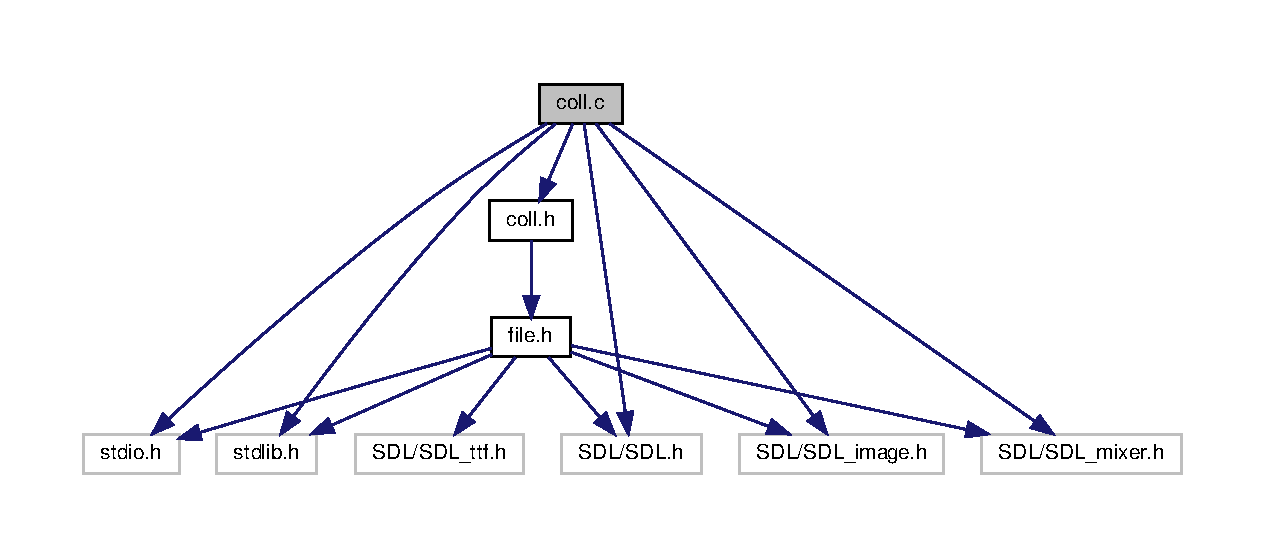
\includegraphics[width=350pt]{coll_8c__incl}
\end{center}
\end{figure}
\subsection*{Functions}
\begin{DoxyCompactItemize}
\item 
\mbox{\Hypertarget{coll_8c_a9ec79b71532402381966fc93325d3e52}\label{coll_8c_a9ec79b71532402381966fc93325d3e52}} 
S\+D\+L\+\_\+\+Color {\bfseries Get\+Pixel} (S\+D\+L\+\_\+\+Surface $\ast$p\+Surface, int x, int y)
\item 
\mbox{\Hypertarget{coll_8c_a4d896b0a63311c54b1e67adb9fd914e5}\label{coll_8c_a4d896b0a63311c54b1e67adb9fd914e5}} 
int {\bfseries collision} (\hyperlink{structperso}{perso} $\ast$\hyperlink{structperso}{perso}, \hyperlink{structmaps}{maps} map)
\end{DoxyCompactItemize}


\subsection{Detailed Description}
collision parfaite $\ast$ 


\begin{DoxyItemize}
\item $\ast$ \begin{DoxyAuthor}{Author}
Dires $\ast$ 
\end{DoxyAuthor}
\begin{DoxyDate}{Date}
Apr 28, 2019 $\ast$ $\ast$ collision parfaite $\ast$ 
\end{DoxyDate}

\end{DoxyItemize}
\hypertarget{jeu_8c}{}\section{jeu.\+c File Reference}
\label{jeu_8c}\index{jeu.\+c@{jeu.\+c}}


l\textquotesingle{}affichage du jeu $\ast$  


{\ttfamily \#include $<$stdio.\+h$>$}\newline
{\ttfamily \#include $<$S\+D\+L/\+S\+D\+L.\+h$>$}\newline
{\ttfamily \#include $<$time.\+h$>$}\newline
{\ttfamily \#include $<$math.\+h$>$}\newline
{\ttfamily \#include $<$S\+D\+L/\+S\+D\+L\+\_\+image.\+h$>$}\newline
{\ttfamily \#include \char`\"{}file.\+h\char`\"{}}\newline
{\ttfamily \#include \char`\"{}scrolling.\+h\char`\"{}}\newline
{\ttfamily \#include \char`\"{}per.\+h\char`\"{}}\newline
{\ttfamily \#include \char`\"{}coll.\+h\char`\"{}}\newline
{\ttfamily \#include \char`\"{}ennemi.\+h\char`\"{}}\newline
{\ttfamily \#include \char`\"{}object.\+h\char`\"{}}\newline
Include dependency graph for jeu.\+c\+:
\nopagebreak
\begin{figure}[H]
\begin{center}
\leavevmode
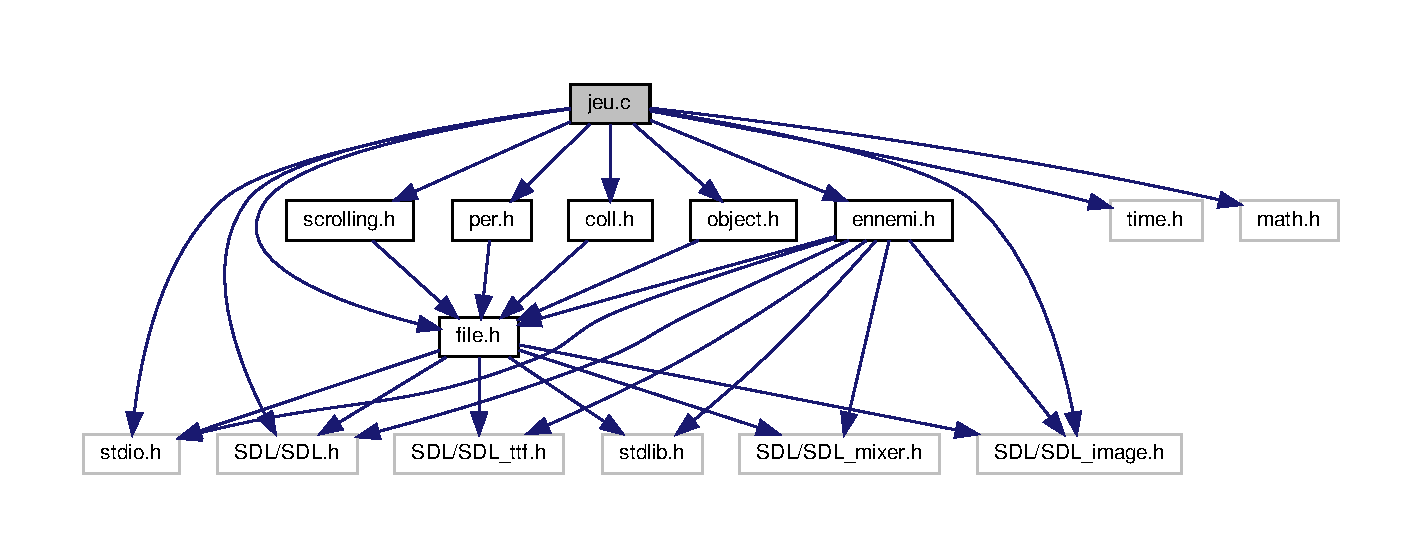
\includegraphics[width=350pt]{jeu_8c__incl}
\end{center}
\end{figure}
\subsection*{Functions}
\begin{DoxyCompactItemize}
\item 
\mbox{\Hypertarget{jeu_8c_a5212944dc69d6229fb839fb8421c07f9}\label{jeu_8c_a5212944dc69d6229fb839fb8421c07f9}} 
void {\bfseries playthegame} ()
\end{DoxyCompactItemize}


\subsection{Detailed Description}
l\textquotesingle{}affichage du jeu $\ast$ 


\begin{DoxyItemize}
\item $\ast$ \begin{DoxyAuthor}{Author}
Dires $\ast$ 
\end{DoxyAuthor}
\begin{DoxyDate}{Date}
May 7, 2019 $\ast$ $\ast$ initialisation et affichage du jeu $\ast$ 
\end{DoxyDate}

\end{DoxyItemize}
\hypertarget{main_8c}{}\section{main.\+c File Reference}
\label{main_8c}\index{main.\+c@{main.\+c}}


le menu du jeu $\ast$  


{\ttfamily \#include $<$stdlib.\+h$>$}\newline
{\ttfamily \#include $<$stdio.\+h$>$}\newline
{\ttfamily \#include $<$S\+D\+L/\+S\+D\+L.\+h$>$}\newline
{\ttfamily \#include $<$S\+D\+L/\+S\+D\+L\+\_\+image.\+h$>$}\newline
{\ttfamily \#include $<$S\+D\+L/\+S\+D\+L\+\_\+mixer.\+h$>$}\newline
{\ttfamily \#include \char`\"{}main.\+h\char`\"{}}\newline
{\ttfamily \#include \char`\"{}file.\+h\char`\"{}}\newline
Include dependency graph for main.\+c\+:
\nopagebreak
\begin{figure}[H]
\begin{center}
\leavevmode
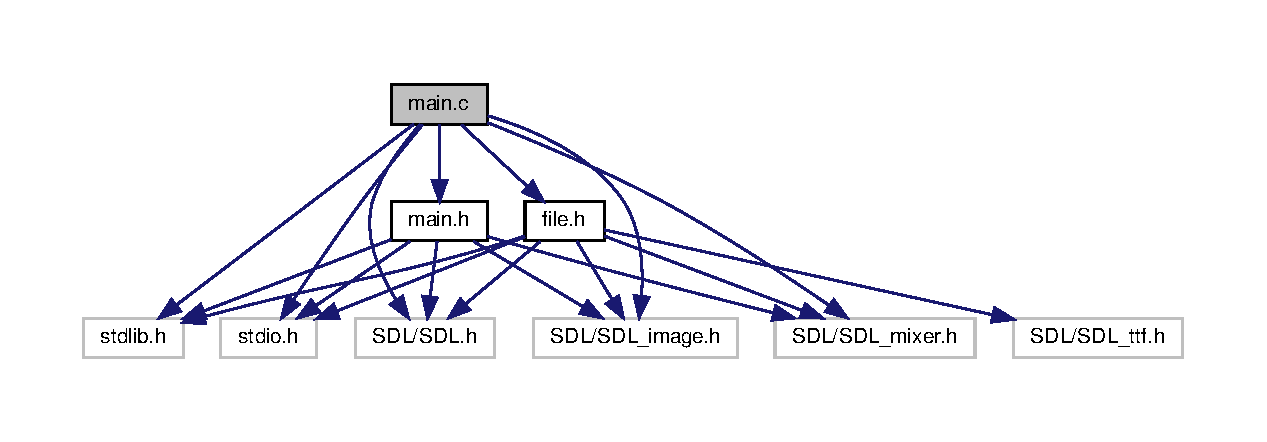
\includegraphics[width=350pt]{main_8c__incl}
\end{center}
\end{figure}
\subsection*{Functions}
\begin{DoxyCompactItemize}
\item 
\mbox{\Hypertarget{main_8c_a0ddf1224851353fc92bfbff6f499fa97}\label{main_8c_a0ddf1224851353fc92bfbff6f499fa97}} 
int {\bfseries main} (int argc, char $\ast$argv\mbox{[}$\,$\mbox{]})
\end{DoxyCompactItemize}


\subsection{Detailed Description}
le menu du jeu $\ast$ 


\begin{DoxyItemize}
\item $\ast$ \begin{DoxyAuthor}{Author}
Dires $\ast$ 
\end{DoxyAuthor}
\begin{DoxyDate}{Date}
May 8, 2019 $\ast$ $\ast$ affichage du menu du jeu $\ast$ 
\end{DoxyDate}

\end{DoxyItemize}
%--- End generated contents ---

% Index
\backmatter
\newpage
\phantomsection
\clearemptydoublepage
\addcontentsline{toc}{chapter}{Index}
\printindex

\end{document}
